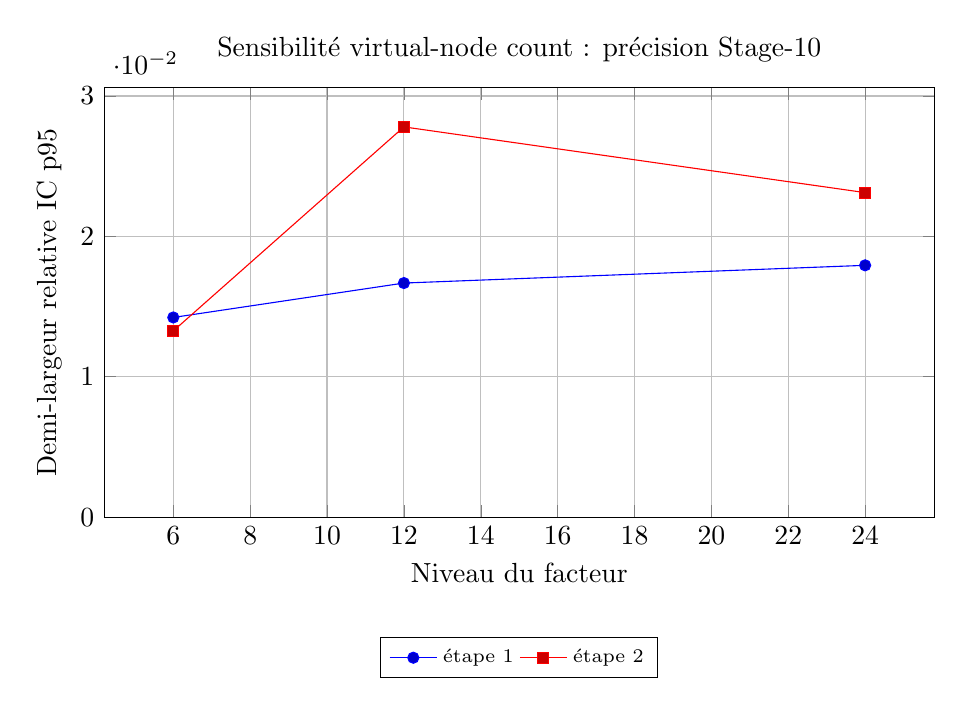
\begin{tikzpicture}
\begin{axis}[width=\linewidth,
height=0.58\linewidth,
title={Sensibilité virtual-node count : précision Stage-10},
xlabel={Niveau du facteur},
ylabel={Demi-largeur relative IC p95},
grid=major,
legend style={font=\scriptsize,at={(0.5,-0.28)},anchor=north,legend columns=2},
ymin=0]
\addplot+[mark=*] coordinates {(6.0,0.014224603883711424) (12.0,0.016675873320203795) (24.0,0.017938439828675615)};
\addlegendentry{étape 1}
\addplot+[mark=square*] coordinates {(6.0,0.013265607159975728) (12.0,0.02780124142449081) (24.0,0.023118318486393095)};
\addlegendentry{étape 2}
\end{axis}
\end{tikzpicture}
